\section{Motivación y Antecedentes} \label{sect:motivacion}

En la sociedad actual se hace imprescindible que las empresas posean una pagina web; el mundo que hoy conocemos se basa en Internet y es en este donde la gente busca las respuestas a sus inquietudes cotidianas. Actualmente en el mundo existen casi el doble de \textit{smartphones} que computadores personales \cite{DGT} y según los resultados obtenidos en una encuesta realizada por Google en cunjunto con IPSOS OTX mediaCT al final del 2010, aparte de recibir y hacer llamadas, las actividades más realizadas en los teléfonos inteligentes son navegar en Internet, el uso de motores de búsquedas y en tercer lugar el uso de aplicaciones \cite{TMM}. Para las empresas, ya no sólo es necesario estar en la web, deben estar al alcance de los teléfonos inteligentes.

Los \textit{smartphones} han llegado a ser parte de la vida de las personas y son dispositivos mucho mas personales que una computadora portátil o de escritorio, estos teléfonos han penetrado hasta el punto que muchos usuarios raramente se separan de sus equipos móviles durante el día. Tomando en cuenta esto y las proyecciones de negocio de \textit{Tuguia.de}; de ser la principal guía de comercios y locales del país, se hace necesario el desarrollo de un mecanismo para que los usuarios puedan acceder a la información del portal desde sus celulares y así hacer de \textit{Tuguia.de} un servicio 24/7, accesible desde cualquier momento y lugar.

Conscientes de la influencia en el éxito de \textit{Tuguia.de} que puede tener la versión móvil de la guía, se decide emprender un desarrollo que permita llevar la aplicación a los celulares inteligentes, sin embargo, existen varias alternativas a considerar si se desea establecer presencia de un negocio en los dispositivos móviles; aplicaciones nativas, aplicaciones híbridas o multiplataforma y paginas web diseñadas específicamente celulares.

Las aplicaciones nativas, llevan este nombre porque son desarrollos implementados en el lenguaje nativo del dispositivo, gracias a esto, sacan el mejor rendimiento posible del \textit{hardware} del móvil, así que tienen un alto desempeño y permiten acceder a las diferentes características presentes en los teléfonos inteligentes con mayor facilidad, sin embargo, el hecho de necesitar un desarrollo en un lenguaje específico, distinto para cada plataforma eleva los costos y el tiempo de desarrollo. 

Las aplicaciones híbridas permiten escribir código en un solo lenguaje para después exportarlo a código nativo y de esta manera obtener una aplicación que funcione en las múltiples plataformas con un solo desarrollo, es de notar que estas aplicaciones tienen un bajo desempeño si las comparamos con las nativas, ademas en estos entornos multiplataforma se dificulta la tarea de acceder a los diferentes componentes del equipo móvil con efectividad. 

Las páginas web de diseño específico para equipos móviles son sitios web que pueden cambiar la forma en la que muestran su contenido de acuerdo al equipo en el que se esta visualizando y de esta manera aprovechar al máximo las dimensiones de las pantallas de los dispositivos, así se consigue que con un solo desarrollo se obtiene un producto que puede operar en tanto en las computadoras como en equipos móviles, al igual que las otras paginas web éstas se ejecutan en un navegador, por lo que se torna bastante complejo acceder a las características propias de los teléfonos inteligentes de hoy en día. 

Luego de evaluar estas alternativas, la junta directiva de \textit{Tuguia.de} decide que desarrollar una aplicación nativa para su proyecto, a pesar de los costos elevados y los altos tiempos de desarrollo desean que la aplicación sea lo mas extensible posible, no obstante, es necesario determinar cuál sistema operativo móvil es el más adecuado para iniciar las versiones móviles de \textit{Tuguia.de}

Según un estudio realizado para finales del 2012 en los Estados Unidos,\cite{NTD} para el tercer trimestre de ese año la participación de Android en el mercado de teléfonos inteligentes era del 52\%, los resultados de dicho estudió lo podemos observar en la figura \ref{fig:marketshare}.
   
\begin{figure}[h]
	\begin{center}
		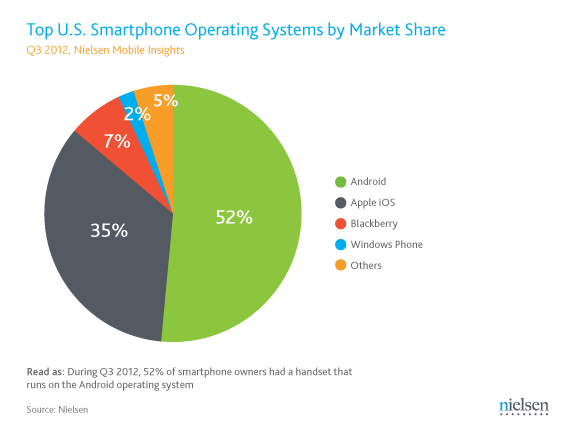
\includegraphics[scale=0.5]{imagenes/Q3-2012-US-Smartphone-OS-market-share.png}
	\end{center}
	\caption{
		\label{fig:marketshare}
		Participación de mercado por sistema operativo móvil \cite{NTD}
	}
\end{figure}

Se hace notable la superioridad de Android sobre los demás sistemas operativos, por lo que es el sistema escogido para iniciar el desarrollo móvil de \textit{Tuguia.de}, pensado en un futuro a corto plazo expandirse al iOS de Apple.
